%TODO: Add support for correlation with complex numbers

\section{Correlation function}

According to \citet{golomb_ref}, the correlation function measures how similar
two phenomena are. If properly normalized, the function ranges from
+1 (identical) to -1 (opposite); 0 meaning completly unrelated phenomena.
If those phenomena are represented as vectors, the correlation can be conceived
as the normalized dot product between those 2 vectors.
In the discrete case where both sequences have the same length, the one in which
this project focus on, the normalized version is defined as follows:

\begin{definition}[Normalized correlation]\label{def:1}

Given $\alpha$ and $\beta$ two vectors of the same length n and $\alpha_{i}$
and $\beta_{i}$ the components of the vectors:

\begin{equation}\label{eq:1}
C(\alpha , \beta)=\frac{(\alpha \cdot  \beta)}{|\alpha||\beta|}=\frac{\sum_{i=1}^{n} \alpha_{i}\beta_{i}}{(\sum_{i=1}^{n} \alpha_{i}^{2})^{\frac{1}{2}}(\sum_{i=1}^{n} \beta_{i}^{2})^\frac{1}{2}}.
\end{equation}
\end{definition}

Notice that in this vector
representation:
\begin{itemize}
  \item Orthogonal vectors have a correlation value of 0 .
  \item Vectors with the same direction and orientation have a correlation
  value of 1.
  \item Vectors with the same direction but opposite orientation have a
  correlation value of -1.
\end{itemize}

Even though the normalized version is a good way to grasp the
concept of the degree of similarity between two phenomen, for the rest of the
document the unnormalized version is going to be used unless it is stated.
This definition of the correlation function have several advantages for our
research as it is simpler and carries the same amount of information while
saving us some computation resources and complexity on our theoretical
analysis. The unnormalized correlation is defined as:

\begin{definition}[Unnormalized correlation]\label{def:2}
  Given $\alpha$ and $\beta$ two vectors of the same length n and $\alpha_{i}$
  and $\beta_{i}$ the components of the vectors:
  \begin{equation}\label{eq:2}
    C(\alpha , \beta) = (\alpha \cdot  \beta) = \sum_{i=1}^n(\alpha \odot \beta)_{i}= \sum_{i=1}^{n} \alpha_{i}\beta_{i}
  \end{equation}

  where "$\odot$" represents the pointwise product of vectors.

\end{definition}

%Adapting this function from vectors to finite digital signals is straight
%forward, as they can be defined in terms of a vector that lives in a vector
%space of dimension equal to the length of the signal.

\begin{figure}[ht!] % [h!] fuerza que el elemento se sitúe
                    % en la posición señalada, en vez de al
                    % comienzo de una página.
\begin{center}
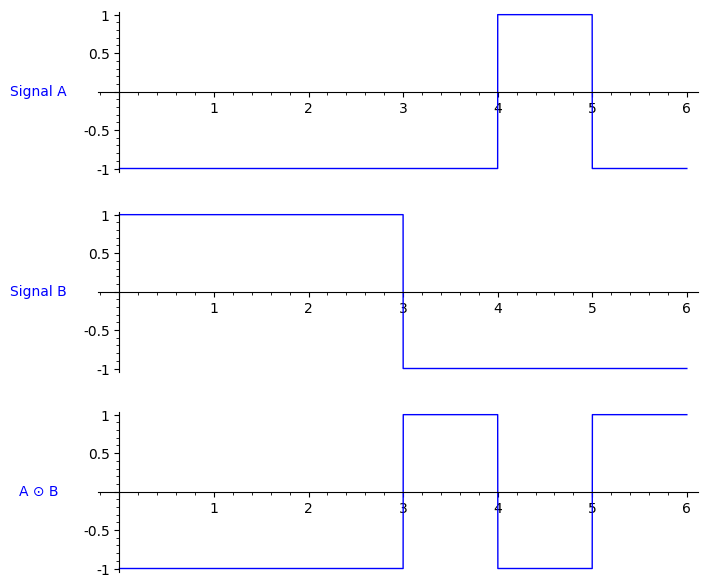
\includegraphics[width=0.7\linewidth]{Chapters/Introduction/signals_correlation}
\end{center}
\caption{A graphical representation of two vectors an their pointwise product
with an unnormalized correlation between them of -2 (-1 -1 -1 +1 -1 +1)}
\label{introduction_signals_hadamard}
\end{figure}

As represented in Figure \ref{introduction_signals_hadamard}, unnormalized
correlation can be performed using only integer arithmetics, multiplication
and addition, thus becoming easier to implement using the resources  avaliable
on a digital device.










\subsection{Autocorrelation function}

Going on with the lecture of \citet{golomb_ref}, the autocorrelation function
is a measure of how the correlation behaves if, for a given sequence, a
circular shift is applied and then correlated with the original sequence for every
possible shift. It is defined for periodic sequences as follows:

\begin{definition}[Autocorrelation]\label{def:3}

Given the function C defined in Equation \eqref{eq:2} and n the length of the
sequence S

\begin{equation}\label{eq:3}
  shift(S, \tau)_i = S_{(i+\tau) \bmod n}
\end{equation}
\begin{equation}\label{eq:4}
  A(S)_{\tau} = C(S, shift(S, \tau)) = \sum_{i=1}^{n}S_{i}S_{(i+\tau) \bmod n}
\end{equation}

\end{definition}

\begin{figure}[ht!] % [h!] fuerza que el elemento se sitúe
                    % en la posición señalada, en vez de al
                    % comienzo de una página.
\begin{center}
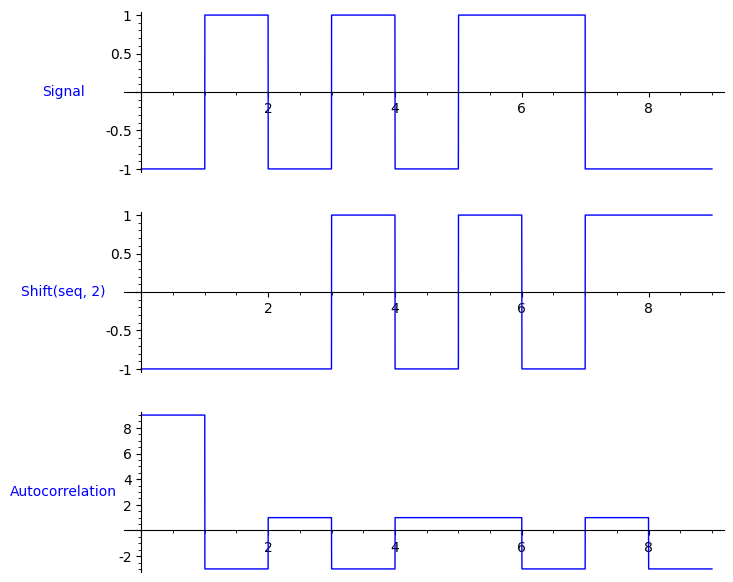
\includegraphics[width=0.7\linewidth]{Chapters/Introduction/signals_autocorrelation}
\end{center}
\caption{A graphical representation of the autocorrelation of a sequence with  a shifted version of itself.}
\label{introduction_signals_autocorrelation}
\end{figure}

An example  is shown in Figure
\ref{introduction_signals_autocorrelation} in which some important properties of
the autocorrelation of sequences can be observed:

\begin{theorem}\label{theorem:1.2.1}
  Given a sequence S, the autocorrelation value for $\tau = 1$ is:
    \begin{equation}
      A(S)_{1}=C(S, S)=\sum_{i=1}^{n}S_{i}^2
    \end{equation}
\end{theorem}

\begin{corollary}
  Given the unnormalized autocorrelation of a sequence, it can be normalized
  normalize by dividing it as follows:
  \begin{equation}
    A'(S)_{\tau} = \frac{A(S)_{\tau}}{A(S)_{1}}
  \end{equation}
\end{corollary}

\begin{proof}
  Using Equations \eqref{eq:1} and \eqref{eq:4}, Equation \eqref{eq:4} can be
  normalized as follows:

    $$A'(S)_{\tau} = C'(S, shift(S, \tau)) = \frac{C(S, shift(S, \tau))}{(\sum_{i=1}^{n} S_{i}^{2})^{\frac{1}{2}}(\sum_{i=1}^{n} S_{i+\tau}^{2})^\frac{1}{2}} = \frac{A(S)_{\tau}}{\sum_{i=1}^{n} S_{i}^{2}} = \frac{A(S)_{\tau}}{A(S)_{1}}$$

  Keep in mind that, even though $S_{i}^2$ and $S_{i+\tau}^2$ aren't the same
  element, the elements of the shifted version are the same as the original
  sequence so the total sum is the same.
\end{proof}

\begin{corollary}\label{autocorrelation:coro:1}
  Given the autocorrelation of a sequence, $A(S)_{1}$ will always be the
  maximum value of the autocorrelation.
\end{corollary}

\begin{property}

  If the components of the original sequence form a field, the components of
  its autocorrelation belong to the same field.

\end{property}

Even though this seems a naive property, this will prove
useful when we introduce the algorithm based in the Fourier Transform to
compute the autocorrelation function.









\subsection{Crosscorrelation function}

The crosscorrelation function measures how a sequence correlates with all
the posible shifts of another sequence. This function is useful to analyze if two
signals can be mistaken one for another by a receiver when delays in time occur.


\begin{definition}[Crosscorrelation]\label{def:4}
  Given C the correlation function defined in Equation \eqref{eq:2}, shift as the function defined in Equation \eqref{eq:3} and n the length of both sequences:
  \begin{equation}\label{eq:7}
    CC(S1, S2)_{\tau} = C(S1, shift(S2, \tau)) = \sum_{i=1}^{n}S1_{i}S2_{(i+\tau) \bmod n}
  \end{equation}
\end{definition}

\begin{figure}[ht!] % [h!] fuerza que el elemento se sitúe
                    % en la posición señalada, en vez de al
                    % comienzo de una página.
\begin{center}
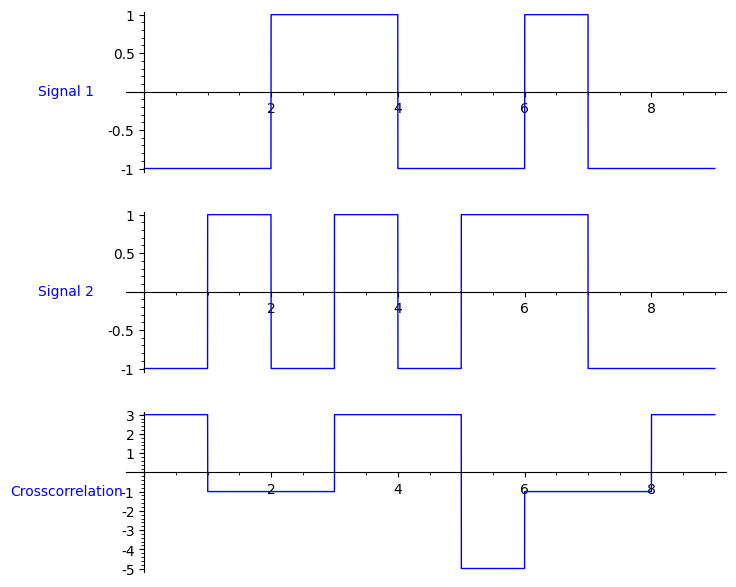
\includegraphics[width=0.7\linewidth]{Chapters/Introduction/signals_crosscorrelation}
\end{center}
\caption{A graphical representation of the crosscorrelation between two sequences.}
\label{introduction_signals_crosscorrelation}
\end{figure}

\begin{definition}\label{lem:1}
  Given a sequence S, the crosscorrelation function  (CC) can bedefined in Equation
  \eqref{eq:7} with the autocorrelation function A defined in Equation \eqref{eq:4}:
  \begin{equation}\label{eq:8}
    CC(S, S) = A(S)
  \end{equation}
\end{definition}












\section{Pseudorandom noise (PN)}

Noise have a different meaning depending on the field of study in which is
used. In our case we are going to work with random vectors,
which are defined as vectors whose components are realizations of independent
and uniform distributed variables\cite{white_noise}.\\

Even though noise in general is usually seen as an unwanted phenomena that
limits the amount of information that can be transmitted through a
channel\cite{shannon_noise}, it is useful to study its properties, such as

%This practical applications exploit an important noise property:

\begin{property}
 The expected value of the autocorrelation of a random vector is zero for
 every component
  where $\tau \neq 0$ \cite{everett}.
\end{property}

Taking a radar as an example, using this property the distance can be computed
just by sending a random sequence in the direction of a target and start
correlating the received signal with the original one. As the autocorrelation
of random vector is different from zero only when the shift is zero, the peak
in the autocorrelation gives in which time instant the signal has returned to
the receiver. With that time instant, the round-trip time can be computed and then
the actual distance using the propagation speed of the wave.\\

In the case of GPS, the restrictions imposed to the random sequence are
stronger. First of all, as several signals will be transmitted in the same
frequency, a set of sequences with good auto and crosscorrelation
properties between them is needed. In other words, the maximum crosscorrelation
function between two given sequences must trend to zero in every component, except
when $\tau = 0$ and both sequences are the same.\\

Random sequences do not guarantee good properties of correlation, even noise
measured from natural phenomena can generate sequences with poor correlation
properties. As stated before, important technologies depend on sequences with
these properties, therefore, it is necessary to develop methods that are
efficient to create sequences with properties similar to those of random in a
deterministic and efficient fashion.\\

This kind of sequences are called Pseudo Noise (PN). Although for most
applications, the off peak autocorrelation and crosscorrelation should be equal to
zero, it is conjetured that such sequence do not exist apart from length four. That
is why pseudo noise are use in practical applications. Then a threshold is defined
so that the system will not mistake intermediate values with the peak in the
autocorrelation.


\begin{figure}[ht!] % [h!] fuerza que el elemento se sitúe
                    % en la posición señalada, en vez de al
                    % comienzo de una página.
\begin{center}
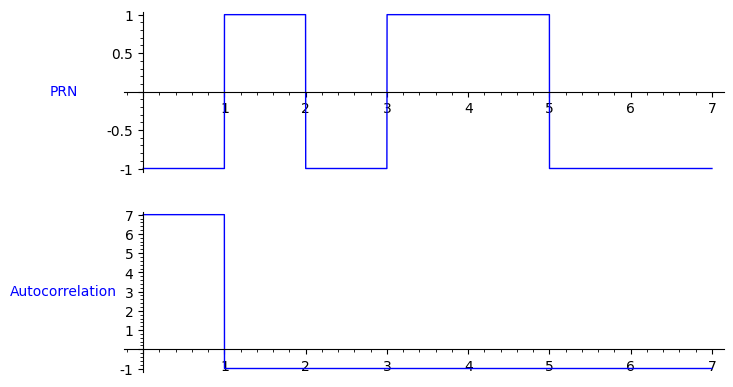
\includegraphics[width=0.7\linewidth]{Chapters/Introduction/signals_prn}
\end{center}
\caption{A pseudorandom noise sequence an it's autocorrelation function.
Notice that this pseudonoise sequence isn't perfect noise.}
\label{introduction_signals_autocorrelation}
\end{figure}

% TODO Define family of sequences

% TODO Define flat autocorrelation
